\documentclass{article}
\usepackage[T1]{fontenc}
\usepackage{lmodern}
\usepackage{graphicx}
\usepackage{amsmath,amssymb}
\usepackage[a4paper,margin=2cm]{geometry}
\usepackage[absolute,overlay]{textpos}
\setlength{\TPHorizModule}{1mm}
\setlength{\TPVertModule}{1mm}
\usepackage[indonesian]{babel}
\usepackage{hyperref}
\setlength{\emergencystretch}{2em}
% unit: Halaman 57

\begin{document}

% === Halaman 57 (llm) ===

\begin{itemize}
  \item Permutasi adalah teknik untuk mengacak susunan bit di dalam sebuah blok bit menghasilkan susunan baru.
\end{itemize}

\vspace{60mm}

\begin{itemize}
  \item Pada gambar di atas, posisi bit-bit di dalam blok input 32-bit dipermutasi menjadi susunan baru.
\end{itemize}

% deskripsi: Diagram permutasi bit yang menunjukkan pemetaan posisi dari blok input 32-bit ke posisi baru di blok output.
% bbox normalisasi: [0.1000, 0.3500, 0.8700, 0.6500]
\begin{textblock*}{161.70mm}(21.00mm,103.95mm)
\noindent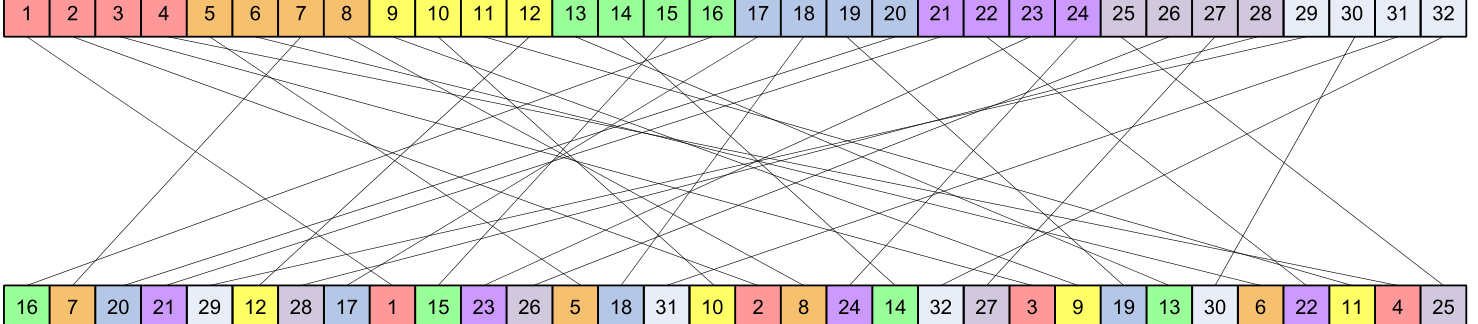
\includegraphics[width=161.70mm,height=89.10mm]{../../images/llm/page_057_img_01.png}%
\end{textblock*}

\end{document}
